\chapter{Vettori e Matrici}
\lecture{2}{9 Sep. 08:00}{Spazi vettoriali}

Sia $(\mathbb{R}^{2},+,\cdot)$ una struttura algebrica (ovvero un insieme non vuoto su cui sono definite delle operazioni), dove $+$ è interna e $\cdot$ è una moltiplicazione di un vettore per uno scalare, $(\mathbb{R}^{2},+,\cdot)$ si chiama \textbf{spazio vettoriale} (e gli elementi di $\mathbb{R}^{2}$ vettori) se valgono le precedenti 8 proprietà.

\begin{es}[Spazi Vettoriali]
	$\mathbb{R}[x] \cong$ Polinomi a coefficienti reali ad un'incognita.\\\\
	$P_{1}(x)=3-x+x^{3} + P_{2}(x)=5x-\frac{7}{2}x^{4}$
	\begin{alignat*}{3}
		3 &{}- x&{}+ x^{3}&  &{}+\\
		  &{}+ 5x&{} &{}- \frac{7}{2}x^{4}&{}=\\
		3 &{}+ 4x&{}+ x^{3}&{}- \frac{7}{2}x^{4}& 
	\end{alignat*}\\
	$\frac{1}{3}P_{1}(x)=1-\frac{1}{3}x+\frac{1}{3}x^{3}$
\end{es}

\begin{definizione}[combinazione lineare]
	Siano $\underline{v}_{1},\underline{v}_{2},...,\underline{v}_{n}, \in V$. Un vettore del tipo $\beta_1 \underline{v} _1+\beta_2 \underline{v} _2+...+\beta_n \underline{v} _n, \beta\in \mathbb{R}$ è combinazione lineare dei vettori $\underline{v} _{1},\underline{v} _{2},...,\underline{v} _{n}$
	\begin{es}
		$3(1,3)+\frac{1}{2}(0,4)+(-1,-1)=(3,9)+(0,2)+(-1,-1)=(2,10)$, questi elementi di $\mathbb{R}^2=(2,10)$ sono combinazione lineare di $(1,3),(0,4),(-1,-1)$ scegliendo $(\beta_1=3, \beta_2=\frac{1}{2}, \beta_3=1)$
	\end{es}
\end{definizione}

\begin{es}[spazi vettoriali]
	\phantom{}\\
    $\mathbb{R}^2, \mathbb{R}^3,...,\mathbb{R}^n$ (Spazio vettoriale dei vettori)\\
    $\mathbb{R}[x], \mathbb{R}[x_1,x_2], \mathbb{R}[x_1,...,x_n]$ (Spazio vettoriale dei polinomi)\\
    $M_{n\times m}, n\wedge m\in \mathbb{N}$ (Spazio vettoriale delle matrici)\\
    \{G\} (Spazio vettoriale dell'elemento nullo)
\end{es}

\begin{es}[elementi neutri negli spazi vettoriali]
	\phantom{}\\
	$\mathbb{R}^2=\underline{0} \Rightarrow (0,0)$\\
	$\mathbb{R}^4=\underline{0} \Rightarrow (0,0,0,0)$\\
	$M_{3\times3}=\underline{0} \Rightarrow 
	\begin{bmatrix}
    0 & 0 & 0 \\
	0 & 0 & 0 \\
	0 & 0 & 0
	\end{bmatrix}$
\end{es}

\section{Proprietà valide negli spazi vettoriali}

\begin{proposizione}
	Sia $V$ uno spazio vettoriale qualunque, $\forall\beta\in\mathbb{R}, \beta 0=0$\\
    \begin{dimostrazione}
    	\phantom{}\\
    	$\beta \underline{0}=\beta(\underline{0}+\underline{0})=\beta \underline{0}+\beta \underline{0}$\\
    	$\beta \underline{0}=\beta \underline{0}+\beta \underline{0}$, esiste l'opposto di $\beta \underline{0}$ e lo chiamiamo $OPP$\\
    	$\beta \underline{0}+ OPP=(\beta \underline{0}+\beta \underline{0})+OPP$\\
    	$\underline{0}=\beta \underline{0}+(\beta \underline{0}+OPP)$\\
    	$\underline{0}=\beta \underline{0}+\underline{0}\rightarrow \beta \underline{0}=\underline{0}$
    \end{dimostrazione}
\end{proposizione}

\begin{proposizione}
	Sia $V$ uno spazio vettoriale qualunque, $\forall \underline{v}\in V, \underline{v}\cdot0=0$\\
	\begin{dimostrazione}
		\phantom{}\\
		$\underline{v}\cdot0=\underline{v}(0+0)=\underline{v}\cdot0+\underline{v}\cdot0$\\
		$\underline{v}\cdot0=\underline{v}\cdot0+\underline{v}\cdot0$, esiste l'opposto di $\underline{v}\cdot0$ e lo chiamiamo $OPP$\\
		$\underline{v}\cdot0+ OPP=(\underline{v}\cdot0+\underline{v}\cdot0)+OPP$\\
		$0=\underline{v}\cdot0+(\underline{v}\cdot0+OPP)$\\
		$0=\underline{v}\cdot0+0\rightarrow \underline{v}\cdot0=0$
	\end{dimostrazione}
\end{proposizione}

\begin{proposizione}
	Sia $V$ uno spazio vettoriale qualunque, l'opposto di $\underline{v}\cdot0$ è $(-1)\underline{v}$\\
	\begin{dimostrazione}
		\phantom{}\\
		$\underline{v}+(-1)\underline{v}=0$\\
		$\underline{v}+(-1)\underline{v}=1\cdot \underline{v}+(-1)\underline{v}=(1-1)\underline{v}=0\cdot \underline{v}=0$, per la proposizione III.2
	\end{dimostrazione}
\end{proposizione}
\newpage
\begin{proposizione}
	Sia $V$ uno spazio vettoriale qualunque, $k\cdot \underline{v}=\underline{0}$, se $k=0$ o $\underline{v}=\underline{0}$\\
	\begin{dimostrazione}
		\phantom{}\\
		Se $k=0$ è vera per la proposizione III.2\\
		Se $k\neq0, \exists \frac{1}{k}\in\mathbb{R}: k\cdot \underline{v}=\underline{0}$\\
		$\frac{1}{k}(k\cdot \underline{v})=\frac{1}{k}\cdot \underline{0}$\\
		$\frac{1}{k}(k\cdot \underline{v})=\underline{0}$ Per la proposizione III.1\\
		$1\cdot \underline{v}=\underline{0}$\\
		$\underline{v}=\underline{0}$
	\end{dimostrazione}
\end{proposizione}

\begin{proposizione}
	In uno spazio vettoriale $V\in\mathbb{R}$ se $\exists \underline{v}\neq 0$ allora $V$ contiene infiniti vettori\\
	\begin{dimostrazione}
		\phantom{}\\
		$1\underline{v}, 2\underline{v}, 3\underline{v},..., n\underline{v}$ facciamo vedere che sono a due a due distinte\\
		$h\cdot \underline{v}=k\cdot \underline{v}$\\
		$(h\cdot \underline{v})+(-1k\cdot \underline{v})=\underline{0}$\\
		$(h-k)\underline{v}=\underline{0}$\\
		$h-k=\underline{0}$ Per la proposizione III.4\\
		$h=k$
	\end{dimostrazione}
\end{proposizione}

\begin{proposizione}
	In uno spazio vettoriale $V$ qualunque, $\underline{v}_{1},\underline{v}_{2},...,\underline{v}_{n}\in V,$ $0\in <\underline{v}_{1},\underline{v}_{2},...,\underline{v}_{n}>$\\
	\begin{dimostrazione}
		\phantom{}\\
		$\exists\beta_1,\beta_2,...,\beta_n:\beta_1 \underline{v}_1+\beta_2 \underline{v}_2+...+\beta_n \underline{v}_n=0$\\
		$\beta_1=\beta_2=...=\beta_n=0$\\
		\begin{nota}
			Con il simbolo $<\underline{v}_{1},\underline{v}_{2},...,\underline{v}_{n}>$ o con $\beta(\underline{v}_{1},\underline{v}_{2},...,\underline{v}_{n})$ indichiamo l'insieme delle combinazioni lineari di $\{\underline{v}_{1},\underline{v}_{2},...,\underline{v}_{n}\}$ cioè l'insieme $\{\beta_1 \underline{v}_1+\beta_2 \underline{v}_2+...+\beta_n \underline{v}_n/\beta_i\in\mathbb{R}\}$
		\end{nota}
	\end{dimostrazione}
	\begin{es}
		\phantom{}\\
		$(0,4)\in<(2,6),(0,4),(-7,2)>?$\\
		Si, infatti basta scegliere $\beta_1\wedge\beta_3=0, \beta_2=1$\\\\
		$(-1,-3)\in<(2,6),(0,4),(-7,2)>?$\\
		Si, $\beta_1\wedge\beta_2=0, \beta_3=-\frac{1}{2}$\\\\
		$(-5,8)\in<(2,6),(0,4),(-7,2)>?$\\
		$(-5,8)=\beta_1(2,6)+\beta_2(0,4)+\beta_3(-7,2)=(2\beta_1-7\beta_3,6\beta_1+4\beta_2+2\beta_3)$\\
		\[
        	\left\{
        	\setlength\arraycolsep{0pt}
    		\begin{array}{ r @{{}={}} r  >{{}}c<{{}} r  >{{}}c<{{}}  r }
			-5 & 2\beta_1 & &          &-& 7\beta_3\\
 			8  & 6\beta_1 &+& 4\beta_2 &+& 2\beta_3\\
			\end{array}
			\right.
		\]
		$\beta_1=1,\beta_2=0,\beta_3=1$
	\end{es}
\end{proposizione}
\leavevmode\\
In generale, l'insieme delle combinazioni lineari $<\underline{v}_{1},\underline{v}_{2},...,\underline{v}_{n}>\subseteq V$. Quindi ogni vettore di V è combinazione lineare di $<\underline{v}_{1},\underline{v}_{2},...,\underline{v}_{n}>$ e si dice che $<\underline{v}_{1},\underline{v}_{2},...,\underline{v}_{n}>$ sono \textbf{generatori} di V.
\begin{es}
	\phantom{}\\
	$\underline{v}_1=(1,2,0,3), \underline{v}_2=(\pi,e,0,-55), \underline{v}_3=(\log_2 3,\sin 8,0,0)$\\\\
	$\underline{v}_1, \underline{v}_2, \underline{v}_3$ generano $\mathbb{R}^4$?\\
	No perché: $\beta_1(1,2,0,3)+\beta_2(\pi,e,0,-55)+\beta_3(\log_2 3,\sin 8,0,0)/\beta_i\in\mathbb{R}$\\
	$(0,0,1,0)$ non è combinazione lineare di $\underline{v}_1,\underline{v}_2,\underline{v}_3$ (In ogni vettore, il terzo elemento è 0, e qualcosa per 0 fa sempre 0)\\\\
\end{es}
\begin{es}
	$P_1(x)=3-x^4, P_2(x)=x+77x^7$\\
	$x^8\in<P_1(x), P_2(x)>$?\\
	No perché non contiene polinomi di grado maggiore a 7.
\end{es}
\begin{es}
	$(1,3)\in\mathbb{R}^2$ genera $\mathbb{R}^2$?\\
	No, perché: $\{\beta(1,3)/\beta_i\in\mathbb{R}\}=\{(\beta,3\beta)/\beta\in\mathbb{R}\}$\\
	$\beta=1\rightarrow(1,3)$ non possiamo generare $(1,1)$
\end{es}
\begin{es}
	$(1,0),(0,1)$ generano $\mathbb{R}^2$?\\
	Si, perché: $(a,b)=?(1,0)+?(0,1)=\beta_1(1,0)+\beta_2(0,1)=(\beta_1,\beta_2)$\\
	$<(1,0),(0,1)>\in\mathbb{R}^2$
\end{es}
\begin{es}
	$(1,0),(0,1),(55,\frac{1}{2})$ generano $\mathbb{R}^2$?\\
	Si, perché: $(a,b)=?(1,0)+?(0,1)+?(55,\frac{1}{2})=\beta_1(1,0)+\beta_2(0,1)+\beta_3(55,\frac{1}{2})$\\
	$<(1,0),(0,1),(55,\frac{1}{2})>\in\mathbb{R}^2$
\end{es}

Come vediamo, se un insieme di vettori ha cardinalità minore della dimensione dello spazio a cui appartengono, allora possiamo immediatamente concludere che l'insieme assegnato non è un sistema di generatori (come visto nel caso polinomiale precedente).\footnote{\href{https://www.youmath.it/lezioni/algebra-lineare/matrici-e-vettori/678-sistema-di-generatori-di-uno-spazio-vettoriale.html}{youmath}} Mentre più avanti, con il concetto di dimensione di spazio vettoriale, sarà più facile capire come verificare se un insieme è generatore.

\begin{nota}
	Se ad un insieme di generatori se ne aggiunge un altro, l'insieme risultante è anch'esso un generatore. Cioè se $\underline{v}_1,...,\underline{v}_n$ genera V allora anche $\underline{v}_1,...,\underline{v}_n,\underline{w}$ diventa generatore.
	\begin{dimostrazione}
		Per ipotesi $V=<\underline{v}_1,...,\underline{v}_n>\phantom{1}\subseteq\phantom{1}<\underline{v}_1,...,\underline{v}_n,\underline{w}>\phantom{1}\subseteq\phantom{1} V$\\
		Dato che $<\underline{v}_1,...,\underline{v}_n,\underline{w}>$ è incluso in V e include V, allora $<\underline{v}_1,...,\underline{v}_n,\underline{w}>$ è V\\
		\begin{es}
			\phantom{}\\
			In $\mathbb{R}^3$, $(0,0,1),(1,0,0),(0,1,0)$ generano $\mathbb{R}^3$\\
			In $\mathbb{R}^1$, $(1)$ genera $\mathbb{R}^1$\\
			In $\mathbb{R}^n$, $(1,0,...,0),(0,1,...,0),(0,0,...,1)$ generano $\mathbb{R}^n$\\
			In $\{G\}$, $G$(vettore nullo) genera $\{G\}$ 
		\end{es}
	\end{dimostrazione}
\end{nota}

Un \textbf{Sistema di vettori} è un insieme in cui contano l'ordine degli elementi e anche le eventuali ripetizioni, e si indica così: $[\underline{v}_1,...,\underline{v}_n]$
\begin{es}
	\phantom{}\\
	$\{(1,0),(0,1),(3,5)\}$ 3 elementi\\
	$\{(1,0),(1,0),(3,5)\}$ 2 elementi $=\{(1,0),(3,5)\}=\{(3,5),(1,0)\}$\\
	$[(1,0),(0,1),(3,5)]$ 3 elementi\\
	$[(1,0),(1,0),(3,5)]$ 3 elementi $\neq[(1,0),(3,5)]\neq[(3,5),(1,0)]$ 
\end{es}
\begin{nota}
$\underline{v}_1=(1,2,3), \underline{v}_2=(0,44,44), \underline{v}_3=(2,4,6)$\\
Esistono varie combinazioni lineari per esprimere gli elementi soprastanti come vettore nullo. Un metodo banale è porre $\beta_1=0,\beta_2=0,\beta_3=0 \longrightarrow 0\cdot(1,2,3),0\cdot(0,44,44), 0\cdot(2,4,6)$\\
Un altro modo sarebbe porre $\beta_1=-2,\beta_2=0,\beta_3=1$
\end{nota}

\section{Dipendenza lineare}
$[\underline{v}_1,...,\underline{v}_n]$ si dice \textbf{linearmente dipendente} se e soltanto se $[0\cdot \underline{v}_1,...,0\cdot \underline{v}_n]$ non è l'unico modo per esprimere $\underline{0}$ come combinazione lineare di $[\underline{v}_1,...,\underline{v}_n]$\\
$[\underline{v}_1,...,\underline{v}_n]$ Si dice \textbf{linearmente indipendente} se e soltanto se $[0\cdot \underline{v}_1,...,0\cdot \underline{v}_n]$ è l'unico modo per esprimere $\underline{0}$ come combinazione lineare di $[\underline{v}_1,...,\underline{v}_n]$

\begin{proposizione}
	Sia V uno spazio vettoriale qualunque e $\underline{v}_1,...,\underline{v}_n$ contiene almeno una coppia di vettori proporzionali, il sistema è linearmente dipendente.
	\begin{es}
		\phantom{text}\\
		$[(2,4),(4,8)]=\underline{0}$\\
		essendo $(4,8)$ il doppio di $(2,4)$ basta porre $\beta_1$ uguale a -2\\
		$[-2\cdot(2,4)+1\cdot(4,8)]=(0,0)$
	\end{es}	
\end{proposizione}

\begin{es}
	$\underline{v}_1=\begin{bmatrix}
		e           & \pi\\
		\frac{1}{2} & \cos \delta
	\end{bmatrix}, \underline{v}_2=\begin{bmatrix}
		0 & 0\\
		0 & 0
	\end{bmatrix}, \underline{v}_3=\begin{bmatrix}
		10^4   & 10^7\\
		10^-31 & 10^0
	\end{bmatrix}$\\\\
	$[\underline{v}_1,\underline{v}_2,\underline{v}_3]$ è linearmente dipendente perché se ci facciamo caso, qualsiasi valore di $\beta$ mettiamo davanti a $\underline{v}_2$ il risultato sarà sempre un vettore con elementi nulli, mentre per $\underline{v}_1$ e $\underline{v}_2$ basta porre il coefficiente di beta uguale a 0.
\end{es}

\begin{es}
	$[(1,0),(0,1)]$ è linearmente indipendente perché gli unici coefficienti di beta possibili sono 0
\end{es}

\begin{es}
	$[(1,0),(0,1),(3,5)]$ è linearmente dipendente perché $(3,5)$ è proporzionale a $(1,0)$ e $(0,1)$\\
	Un modo per esprimere il vettore nullo è: $-3(1,0)+[-5(0,1)]+1(3,5)$
\end{es}

\section{Teorema di caratterizzazione dei sistemi di vettori linearmente dipendenti}

\begin{teorema}\label{caratterizzazione}
	$[v_1,...,v_n]$ lin. dipendenti $\Longleftrightarrow $ Almeno un vettore è combinazione lineare degli altri\\
	\begin{dimostrazione}[da destra a sinistra]
		\phantom{}\\
		Se $\underline{v}_n\in <\underline{v}_1,...,\underline{v}_{n-1}>$\\
		$\underline{v}_n=\beta_1 \underline{v}_1+...+\beta_{n-1} \underline{v}_{n-1}$\\
		$0=\beta_1 \underline{v}_1+...+\beta_{n-1}\underline{v}_{n-1}+(-1)\underline{v}_n \Longrightarrow [\underline{v}_1,...,\underline{v}_n]$ linearmente dipendente 
	\end{dimostrazione}
	\begin{dimostrazione}[da sinistra a destra]
		\phantom{}\\
		Per ipotesi $\exists\beta_1,...,\beta_n$ non tutti nulli tale che $0=\beta_1 \underline{v}_1+...+\beta_n \underline{v}_n$\\
		se $\beta_n\neq 0\Longrightarrow  \underline{v}_n=\frac{1}{\beta_n}(-\beta_1 \underline{v}_1,...,-\beta_{n-1}\underline{v}_n-1)=(-\frac{\beta_1}{\beta_n})\underline{v}_1+...+(-\frac{\beta_{n-1}}{\beta_n})\underline{v}_{n-1}$
	\end{dimostrazione}
\end{teorema}

\begin{corollario}
	$[\underline{v}_1,\underline{v}_2]$ linearmente dipendenti $\Longleftrightarrow$ Almeno un vettore è combinazione lineare dell'altro $\Longleftrightarrow $ sono proporzionali
\end{corollario}

\begin{es}
	$[
		\begin{pmatrix}
			1 & 2\\
			3 & 4
		\end{pmatrix},
		\begin{pmatrix}
			e           & \pi\\
			\frac{1}{2} & 0
		\end{pmatrix}
	]$ non sono proporzionali $\Longrightarrow$ linearmente indipendenti
\end{es}

\begin{esercizio}
	Sia $P_1(x)=x^{29}+x^9+x^2023$\\\\
	Determinare $P_2(x),P_3(x)$ tali che: $[P_1(x),P_2(x)]$ lin. indipendenti e $[P_1(x),P_3(x)]$ lin. dipendenti\\
	$P_2(x)$ basta che non sia proporzionale a $P_1(x)$: $P_2(x)=2$\\
	$P_3(x)$ basta che sia proporzionale a $P_1(x)$: $P_3(x)=0$ oppure $P_3(x)=2x^{29}+2x^9+2x^2023$
\end{esercizio}

\begin{osservazione}
	$\underline{v}\in V$\\\\
	$\underline{v}$ è linearmente dipendente se $\underline{v}=\underline{0}$\\
	infatti $\beta \underline{v}=\beta \underline{0}=\underline{0}, \forall\beta\in\mathbb{R}$\\\\
	$\underline{v}$ è linearmente indipendente se $\underline{v}\neq \underline{0}$\\
	infatti $\beta \underline{v}=\underline{0}\Longleftrightarrow \beta=0$
\end{osservazione}

\begin{center}
	\begin{tabular}{ccc}
		$V=\mathbb{R}$ & Lin. indipendenti & Generatori \\
			 $[(1,0)]$ &                SI & NO \\
	   $[(1,0),(0,1)]$ &                SI & SI \\
 $[(1,0),(0,1),(0,5)]$ &                NO & SI \\
	   $[(1,0),(3,0)]$ &                NO & NO \\
 \end{tabular}
\end{center}

\begin{figure}[H]
	\centering
	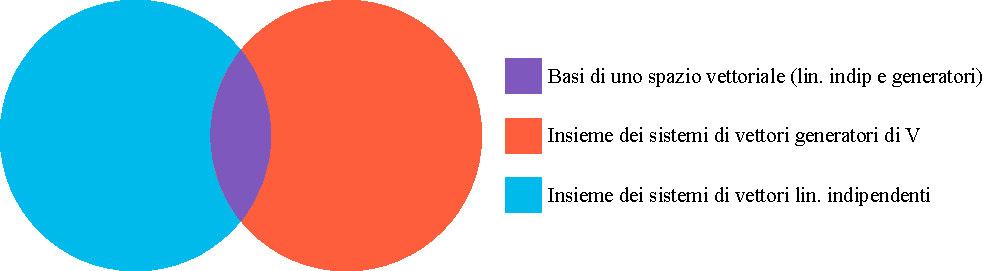
\includegraphics[height=0.24\textwidth]{Figures/insiemi sistemi vettoriali.pdf}
	\caption[Caption]{Insiemi dei sistemi vettoriali}
	\label{fig:insiemisistemivett}
\end{figure}

\section{Basi di uno spazio vettoriale}

Un sistema ordinato $[\underline{v}_1,...,\underline{v}_n]$ si dice base di V se i vettori sono linearmente indipendenti e generano V.
\begin{nota}
	\phantom{}\\
	$[(1,0),(0,1)]$ base canonica di $\mathbb{R}$\\
	$[(1,0,0),(0,1,0),(0,0,1)]$ base canonica di $\mathbb{R}^3$\\
	$\{G\}=\{\underline{0}\}$ Non ha basi, perché i vettori sono linearmente dipendenti ($n\cdot G=0/\forall n\in \mathbb{R}$)\\
	$P[x]$ Non ha basi, perché non è finitamente generato
\end{nota}

Data una base, per trovarne una nuova, basta cambiare l'ordine dei vettori contenuti in essa, oppure sostituire qualche vettore con uno proporzionale \textbf{non nullo}.

\begin{es}
	\phantom{}\\
	$B^{'}=[(1,0,0),(0,1,0),(0,0,1)]$\\
	$B^{''}=[(1,0,0),(0,0,1),(0,1,0)]$\\
	Queste sono due basi diverse di $\mathbb{R}^3$, dove nel secondo caso abbiamo solo cambiato l'ordine di $\underline{v}_2$ con $\underline{v}_3$\\
	$[(0,1,0),(0,0,-1),(2023,0,0)]$\\
	Invece qui abbiamo sia cambiato l'ordine vettoriale e sia proporzionato gli elementi con diversi coefficienti
\end{es}

\begin{nota}[DIP+1=DIP]
	Se ad un sistema linearmente dipendente si aggiunge un vettore, il sistema finale è linearmente dipendente
	\begin{dimostrazione}
		$[\underline{v}_1,...,\underline{v}_n]$ linearmente dipendente\\
		$\exists\beta_1,...,\beta_n$ non tutti nulli tali che $\underline{0}=\beta_1\underline{v}_1+...+\beta_n\underline{v}_n$\\
		$\underline{0}=\beta_1\underline{v}_1+...+\beta_n\underline{v}_n+0\underline{w}$\\
		$[\underline{v}_1,...,\underline{v}_n,\underline{w}]$ linearmente dipendente $\forall\underline{w}\in$V\\
		Quindi in parole povere, se già abbiamo un sistema linearmente dipende e aggiungiamo un vettore a caso, possiamo sempre annullarlo moltiplicando per 0 e non cambia niente in termini di dipendenza
	\end{dimostrazione}
\end{nota}

\begin{nota}[INDIP-1=INDIP]
	Se ad un sistema linearmente indipendente si toglie un vettore, il sistema finale è linearmente indipendente
	\begin{dimostrazione}
		$[\underline{v}_1,...,\underline{v}_{n-1}]/n\geq 1$ linearmente indipendente\\
		Per assurdo, può essere $[\underline{v}_1,...,\underline{v}_{n-2}]/n\geq 2$ linearmente dipendente? No, in base al principio DIP+1=DIP dovrebbe essere linearmente dipendente anche il sistema di partenza
	\end{dimostrazione}
\end{nota}

\begin{nota}[Sistema indipendente massimale]
	Un sistema indipendente si dice indipendente massimale, se appena si aggiunge un vettore, l'indipendenza si perde
\end{nota}

\begin{nota}[Sistema minimale di generatori]
	Un sistema di generatori si dice minimale di generatori, se appena si toglie un vettore, il sistema risultante non è più generatore
\end{nota}
\section{Teorema di caratterizzazione delle basi}
\begin{teorema}
	Sia V uno spazio vettoriale non banale. Un sistema ordinato di vettori $B=[\underline{e}_1,...,\underline{e}_n]$ di V è una base ordinata se e solo se vale una delle seguenti condizioni:
	\begin{itemize}
		\item $\Longleftrightarrow$ il sistema è indipendente massimale
		\item $\Longleftrightarrow$ il sistema è minimale di generatori
		\item $\Longleftrightarrow$ ogni vettore di V, si può esprimere come combinazione lineare dei vettori di B, in un solo modo
	\end{itemize}
	\begin{dimostrazione}[da destra a sinistra]
		\phantom{}\\
		$B=[\underline{e}_1,...,\underline{e}_n]$ per ipotesi si sa già essere generatore, bisogna dimostrare quindi che sia linearmente indipendente. Il sistema B è linearmente indipendente, perché essendo ogni vettore esprimibile in un solo modo, anche $\underline{0}$ si può esprimere in un solo modo. Quindi B è linearmente indipendente
	\end{dimostrazione}
	\begin{dimostrazione}[da sinistra a destra]
		\phantom{}\\
		$B=[\underline{e}_1,...,\underline{e}_n]$ è una base di V, quindi supponiamo che:\\
		$\underline{v}=\beta_1 \underline{e}_1+...+\beta_n \underline{e}_n$\\
		$\underline{v}=\gamma_1 \underline{e}_1+...+\gamma_n \underline{e}_n$\\
		Sottraendo membro a membro: $\underline{0}=(\beta_1-\gamma_1)\underline{e}_1+...+(\beta_n-\gamma_n)\underline{e}_n$\\
		Essendo per ipotesi, linearmente indipendente: $\beta_1-\gamma_1=0, \beta_n-\gamma_n=0$
	\end{dimostrazione}
\end{teorema}

\begin{proposizione}
	\phantom{}\\
	$B^{\phantom{'}}=[(1,0,0),(0,1,0),(0,0,1)]\swarrow$\\
	\phantom{texttt}$(a,b,c)=a(1,0,0)+b(0,1,0)+c(0,0,1)$\\\\
	$B^{'}=[(0,1,0),(0,0,1),(1,0,0)]\swarrow$\\
	\phantom{texttt}$(a,b,c)=b(0,1,0)+c(0,0,1)+a(1,0,0)$\\\\
	$B^{"}=[(0,1,0),(0,0,-1),(2023,0,0)]\swarrow$\\
	\phantom{texttt}$(a,b,c)=b(0,1,0)-c(0,0,-1)+\frac{a}{2023}(2023,0,0)$\\\\
	In qualunque spazio vettoriale V che possegga una base, un vettore $\underline{v}$ si può esprimere come: $\underline{v}=\beta_1\underline{e}_1+...+\beta_n\underline{e}_n$. I coefficienti $\beta_1,...,\beta_n$ individuano univocamente $\underline{v}$ e prendono anche il nome di componenti di $\underline{v}$ rispetto alla base B.
	\begin{es}
		$\underline{v}=(3,10,2023)\in\mathbb{R}^{2}$\\
		Le componenti di $\underline{v}$ rispetto a $B$ sono $(3,10,2023) \swarrow$\\
		$a(1,0,0)+b(0,1,0)+c(0,0,1)=(3,10,2023)$\\
		$\textbf{3}(1,0,0)+\textbf{10}(0,1,0)+\textbf{2023}(0,0,1)=(3,10,2023)$\\\\
		Le componenti di $\underline{v}$ rispetto a $B^{'}$ sono $(10,2023,3) \swarrow$\\
		$b(0,1,0)+c(0,0,1)+a(1,0,0)=(3,10,2023)$\\
		$\textbf{10}(0,1,0)+\textbf{2023}(0,0,1)+\textbf{3}(1,0,0)=(3,10,2023)$\\\\
		Le componenti di $\underline{v}$ rispetto a $B^{"}$ sono $(10,-2023,\frac{3}{2023}) \swarrow$\\
		$b(0,1,0)+c(0,0,-1)+\frac{a}{2023}(2023,0,0)=(3,10,2023)$\\
		$\textbf{10}(0,1,0)-\textbf{2023}(0,0,-1)+\frac{\textbf{3}}{2023}(2023,0,0)=(3,10,2023)$
	\end{es}
	\begin{es}
		$B=[\begin{pmatrix}
			1 & 1\\
			0 & 0
		\end{pmatrix},\begin{pmatrix}
			0 & -2\\
			0 & 0
		\end{pmatrix},\begin{pmatrix}
			0 & 0\\
			1 & 0
		\end{pmatrix},\begin{pmatrix}
			0 & 0\\
			0 & 55
		\end{pmatrix}]$\\
		Calcolare le componenti del vettore $\begin{pmatrix}
			1 & 2\\
			3 & 4
		\end{pmatrix}\in M_{2\times 2}$ rispetto a B:\\
		$\begin{pmatrix}
			1 & 2\\
			3 & 4
		\end{pmatrix}=\beta\begin{pmatrix}
			1 & 1\\
			0 & 0
		\end{pmatrix}+\delta\begin{pmatrix}
			0 & -2\\
			0 & 0
		\end{pmatrix}+\lambda\begin{pmatrix}
			0 & 0\\
			1 & 0
		\end{pmatrix}+\varpi\begin{pmatrix}
			0 & 0\\
			0 & 55
		\end{pmatrix}=\begin{pmatrix}
			\beta   & \beta-2\delta\\
			\lambda & 55\varpi
 		\end{pmatrix}$\\\\
		Quindi $\beta=1, \beta-2\delta=2, \lambda=3, 55\varpi=4$\\
		$\beta=1, \delta=-\frac{1}{2}, \lambda=3, \varpi=\frac{4}{55}$
	\end{es}
	\begin{es}
		Data la base $B^{'}=[(1,2),(3,4)]$ di $\mathbb{R}^2$ calcolare il vettore di componenti $(5,8)$\\
		$\underline{v}=5(1,2)+8(3,4)=(5,10)+(24,32)=(29,42)$
	\end{es}
\end{proposizione}

\begin{definizione}
	Il determinante è una funzione che ha per dominio una matrice quadrata\\
	$\det=M_{n\times n}\Longrightarrow\mathbb{R}$\\
	Calcolo del determinante di una matrice quadrata:\\
	$n=1\Longrightarrow \det(a_{1,1})=a_{1,1}$\\
	$n=2\Longrightarrow \det\begin{pmatrix}
		a_{1,1} & a_{1,2}\\
		a_{2,1} & a_{2,2}
	\end{pmatrix}=(a_{1,1}\cdot a_{2,2})-(a_{1,2}\cdot a_{2,1})$\\
	si può anche capire meglio visualizzando l'operazione come una croce:
	\begin{tabular}{r@{\qquad}r}
		\tikznode{a_{1,1}}{$a_{1,1}$} & \tikznode{a_{1,2}}{$a_{1,2}$} \\[2ex]
		\tikznode{a_{2,1}}{$a_{2,1}$} & \tikznode{a_{2,2}}{$a_{2,2}$} 
	\end{tabular}
	\begin{tikzpicture}[remember picture,overlay,> = stealth',shorten <= 4pt,shorten > = 4pt]
	  \draw[->] (a_{1,1}.east) -- (a_{2,2}.west);
	  \draw[->] (a_{2,1}.east) -- (a_{1,2}.west);
	\end{tikzpicture}
\end{definizione}

\begin{proposizione}[Prima proprietà elementare dei determinanti]
	Data una matrice $M_{n\times n}, \forall n\in\mathbb{N}$ scambiando due righe o due colonne, il determinante cambia segno\\
	\begin{corollario}
		Se la matrice ha due righe o due colonne uguali, $\det=0$
		\begin{dimostrazione}
			$\det\begin{pmatrix}
				1 & 2 & 3 & 4\\
				5 & 6 & 7 & 8\\
				1 & 2 & 3 & 4\\
				e & \frac{1}{2} & e & \frac{1}{3}
			\end{pmatrix}=-\det\begin{pmatrix}
				1 & 2 & 3 & 4\\
				5 & 6 & 7 & 8\\
				1 & 2 & 3 & 4\\
				e & \frac{1}{2} & e & \frac{1}{3}
			\end{pmatrix}=0$\\\\
			Sono state invertite la prima e la terza riga, quindi essendo 0 l'unico numero che moltiplicato per -1 assume lo stesso valore, è l'unica soluzione accettabile
		\end{dimostrazione}
	\end{corollario} 
\end{proposizione}

\begin{lemma}[Steinitz]\label{lemmadisteinitz}
	Sia V uno spazio vettoriale avente $[\underline{e}_1,...,\underline{e}_n]$ come base, e sia $S=[\underline{v}_1,...,\underline{v}_m]$ un sistema di vettori di V. Se $m>n$, il sistema S è linearmente dipendente.\\
	Sia $[\underline{e}_1,...,\underline{e}_n]$ una base di V e sia $S=[\underline{v}_1,...,\underline{v}_h]$ un sistema linearmente indipendente, allora $h\leq n$
	\begin{es}
		$S=[(1,2,3),(\pi,\pi^2,\pi^3),(5,50,500),(\frac{1}{2},\frac{1}{4},\frac{1}{6})]\in\mathbb{R}^3$\\
		$[(1,0,0),(0,1,0),(0,0,1)]$ base canonica di $\mathbb{R}^3$\\
		Il sistema S è linearmente dipendente, per il \ref{lemmadisteinitz}
	\end{es}
\end{lemma}

\begin{teorema}[Equipotenza delle basi]\label{equipotenza}
	Per potenza di un insieme finito si intende il numero dei suoi elementi. Due basi di uno stesso spazio vettoriale hanno lo stesso numero di elementi
	\begin{dimostrazione}
		\phantom{}\\
		\begin{itemize}
			\item[hp] $B=[\underline{e}_1,...,\underline{e}_n],\phantom{1}B^{'}=[\underline{e}_1,...,\underline{e}_m]$ basi di V
			\item[th] $m=n$
		\end{itemize}
		$B$ è una base, $B^{'}$ in particolare è indipendente $\Longrightarrow$ $m\leqslant n$ Per il \ref{lemmadisteinitz}\\
		$B^{'}$ è una base, $B$ in particolare è indipendente $\Longrightarrow$ $n\leqslant m$ Per il \ref{lemmadisteinitz}\\
		Quindi $m=n$
	\end{dimostrazione}
	\begin{esercizio}
		$S=[(1,2,3,4),(\frac{1}{2},\pi,\sin 8, 55)]$ genera $\mathbb{R}^4$?\\
		$S$ genera $\mathbb{R}^4$ se $\forall(a,b,c,d)\in\mathbb{R}^4\phantom{1}\exists\beta,\delta\in\mathbb{R}$ tali che:\\ 
		$(a,b,c,d)=\beta(1,2,3,4)+\delta(\frac{1}{2},\pi,\sin 8, 55)$
		S è indipendente (Lemma di Steinitz \ref{lemmadisteinitz}), S non è una base (Teor. equipotenza delle basi \ref{equipotenza}) $\longrightarrow$ S non è un generatore
	\end{esercizio}
	\begin{osservazione}
		\phantom{}\\
		$[(1,2,3),(1,1,1)]$ Non è una base di $\mathbb{R}^3$ per il \ref{equipotenza}\\
		$[(1,2,3),(0,1,1),(5,55,0),(8,8,8)]$ Non è una base di $\mathbb{R}^3$ perché per il \ref{lemmadisteinitz} sono linearmente dipendenti\\
		$[(1,2,3),(0,1,1),(5,55,0)]$ Se sono linearmente indipendenti allora sono una base di $\mathbb{R}^3$. Come verificarlo?\\
		Se $\det\begin{pmatrix}
			1 & 2 & 3\\
			0 & 1 & 1\\
			5 & 55& 0
		\end{pmatrix}\neq 0$ allora è lin. indipendente
	\end{osservazione}
\end{teorema}

\begin{proposizione}[Dimensione di uno spazio vettoriale]
	\phantom{}\\
	La \textbf{dimensione di uno spazio vettoriale} finitamente generato è uguale al \textbf{numero di vettori che contiene una base} (ovvero \underline{linearmente indipendenti})\\
	$
		\dim V= 
		\begin{cases}
		  0 & \text{se } V=\{\underline{0}\}\\
		  n\degree & \text{di vettori contenuti in una sua base se } V\neq \{\underline{0}\}
		\end{cases}
	$\\\\
	Perché $V\neq\{\underline{0}\}$ (finitamente generato) contiene una base?\\
	Hp: $[\underline{v}_1,...,\underline{v}_n]$ generano V
	\begin{itemize}
		\item[-] Se il sistema è minimale di generatori, allora è una base; altrimenti esistono $n-1$ vettori che generano V
		\item[-] Iterando il ragionamento (togliendo i vettori superflui) si arriva ad una base di V
	\end{itemize}
	\begin{es}
		\phantom{}\\
		$\dim\mathbb{R}=1$\\
		$\dim\mathbb{R}^2=2$\\
		$\dim\mathbb{R}^n=n$\\
		$\dim\{\underline{0}\}=0$\\
		$\dim M_{n\times m}=n\times m$
	\end{es}
\end{proposizione}

\begin{lemma}[conseguenza del lemma di Steinitz]\label{conselemmadisteinitz}
	Sia V uno spazio vettoriale finitamente generato e $\dim V=n>0$\\
	\begin{itemize}
		\item[-] Se $[\underline{v}_1,...,\underline{v}_n]$ è indipendente, allora è anche generatore
		\item[-] Se $[\underline{v}_1,...,\underline{v}_n]$ è generatore, allora è anche indipendente
	\end{itemize}
	\begin{dimostrazione}[INDIP=GEN]
		\phantom{}\\
		$[\underline{v}_1,\underline{v}_2,\underline{v}_3]$ indipendente\\
		$[\underline{v}_1,\underline{v}_2,\underline{v}_3,\underline{w}]$ è dipendente per ogni $w$ \ref{lemmadisteinitz}\\
		$[\underline{v}_1,\underline{v}_2,\underline{v}_3]$ è indipendente massimale\\
		$[\underline{v}_1,\underline{v}_2,\underline{v}_3]$ è una base $\longrightarrow$ indipendente e generatore
	\end{dimostrazione}
	\begin{dimostrazione}[GEN=INDIP]
		\phantom{}\\
		$[\underline{v}_1,\underline{v}_2,\underline{v}_3]$ è generatore di $\mathbb{R}^3$\\
		è per forza minimale, perché altrimenti $\mathbb{R}^3$ avrebbe una base con meno di 3 vettori\\
		$[\underline{v}_1,\underline{v}_2,\underline{v}_3]$ è una base\\
		indipendente e generatore
	\end{dimostrazione}
\end{lemma}

\begin{proposizione}[seconda proprietà elementare dei determinanti]
	\phantom{}\\
	$\beta\det\begin{pmatrix}
		\underline{a}_1\\
		\vdots\\
		\underline{a}_n
	\end{pmatrix}=\det\begin{pmatrix}
		\beta\underline{a}_1\\
		\vdots\\
		\underline{a}_n
	\end{pmatrix};\beta\det\begin{pmatrix}
		\underline{a}_1, \cdots, \underline{a}_n
	\end{pmatrix}=\det\begin{pmatrix}
		\beta\underline{a}_1, \cdots, \underline{a}_n
	\end{pmatrix}$
	\begin{corollario}
		Se in una matrice quadrata troviamo due righe o due colonne proporzionali, il determinante è uguale a 0\\
		$
		\det\begin{pmatrix}
			1  & 2  & 3  & 4 \\
			5  & 6  & 7  & 8 \\
			10 & 20 & 30 & 40\\
			9  & 10 & 11 & 12
		\end{pmatrix}=10\det\begin{pmatrix}
			1  & 2  & 3  & 4 \\
			5  & 6  & 7  & 8 \\
			1  & 2  & 3  & 4 \\
			9  & 10 & 11 & 12
		\end{pmatrix}=10\cdot 0=0
		$\\\\
		$
		\det\begin{pmatrix}
			1  & 2  & 0  & -5\\
			\pi& e  & 0  & 8 \\
			1  & 1  & 0  & 7 \\
			2  & \frac{1}{4} & 0 & 10
		\end{pmatrix}=0
		$ perché $\underline{a}^3=0\underline{a}^{1}=0\underline{a}^{2}=0\underline{a}^{4}$(Colonne)\\\\\\
		$B=\begin{pmatrix}
			1 & 2\\
			3 & 4
		\end{pmatrix}, \det B=-2$\\
		$\det(5B)=\det\begin{pmatrix}
			5\cdot 1 & 5\cdot 2\\
			5\cdot 3 & 5\cdot 4
		\end{pmatrix}=5\cdot 5\det\begin{pmatrix}
			1 & 2\\
			3 & 4
		\end{pmatrix}=25\cdot(-2)=-50$
	\end{corollario}
	\begin{corollario}
		$A\in M_{n\times m}$ e $\beta\in\mathbb{R}\longrightarrow\det(\beta A)=\beta^n\det A$
	\end{corollario}
\end{proposizione}

\newpage

\begin{proposizione}[terza proprietà elementare dei determinanti]
	\phantom{}\\
	$\det\begin{pmatrix}
		\underline{a}_1\\
		\underline{c}_2\\
		\vdots\\
		\underline{c}_n
	\end{pmatrix}+\det\begin{pmatrix}
		\underline{b}_1\\
		\underline{c}_2\\
		\vdots\\
		\underline{c}_n
	\end{pmatrix}=\begin{pmatrix}
		\underline{a}_1+\underline{b}_1\\
		\underline{c}_2\\
		\vdots\\
		\underline{c}_n
	\end{pmatrix}$ (vale anche per le colonne)\\
	\begin{es}
		$\det\begin{pmatrix}
			1 & 0\\
			3 & 4\\
		\end{pmatrix}+\det\begin{pmatrix}
			5 & 6\\
			3 & 4\\
		\end{pmatrix}=\det\begin{pmatrix}
			6 & 6\\
			3 & 4\\
		\end{pmatrix}=6\cdot\det\begin{pmatrix}
			1 & 1\\
			3 & 4\\
		\end{pmatrix}$
	\end{es}
\end{proposizione}

\begin{teorema}[Dipendenza lineare e matrici]
	\phantom{}\\
	$V=\mathbb{R}^n$ se $[\underline{v}_1,\cdots,\underline{v}_n]$ è linearmente indipendente e quindi se e solo se $\det\begin{pmatrix}
		\underline{v}_1\\
		\cdots\\
		\underline{v}_n
	\end{pmatrix}\neq 0$
	\begin{dimostrazione}[da dx a sx, n=4]
		\phantom{}\\
		Se $[\underline{v}_1,\underline{v}_2,\underline{v}_3,\underline{v}_4]$ è linearmente dipendente, allora, almeno uno di essi è combinazione lineare degli altri [teorema di caratterizzazione], quindi supponiamo che $\underline{v}_4=\alpha\underline{v}_1+\beta\underline{v}_2+\gamma\underline{v}_3$\\
		$\det\begin{pmatrix}
			\underline{v}_1\\
			\underline{v}_2\\
			\underline{v}_3\\
			\underline{v}_4
		\end{pmatrix}=\det\begin{pmatrix}
			\underline{v}_1\\
			\underline{v}_2\\
			\underline{v}_3\\
			(\alpha\underline{v}_1+\beta\underline{v}_2)\gamma\underline{v}_3
		\end{pmatrix}=\det\begin{pmatrix}
			\underline{v}_1\\
			\underline{v}_2\\
			\underline{v}_3\\
			\alpha\underline{v}_1+\beta\underline{v}_2
		\end{pmatrix}+\det\begin{pmatrix}
			\underline{v}_1\\
			\underline{v}_2\\
			\underline{v}_3\\
			\gamma\underline{v}_3
		\end{pmatrix}\\
		\det\begin{pmatrix}
			\underline{v}_1\\
			\underline{v}_2\\
			\underline{v}_3\\
			\alpha\underline{v}_1
		\end{pmatrix}+\det\begin{pmatrix}
			\underline{v}_1\\
			\underline{v}_2\\
			\underline{v}_3\\
			\beta\underline{v}_2
		\end{pmatrix}+\det\begin{pmatrix}
			\underline{v}_1\\
			\underline{v}_2\\
			\underline{v}_3\\
			\gamma\underline{v}_3
		\end{pmatrix}=0$
	\end{dimostrazione}
\end{teorema}

\begin{corollario}[relativo alla terza proprietà]
	\phantom{text}\\
	$\det\begin{pmatrix}
		\underline{a}_1+\beta\underline{a}_i\\
		\underline{a}_2\\
		\vdots\\
		\underline{a}_n
	\end{pmatrix}=\det\begin{pmatrix}
		\underline{a}_1\\
		\vdots\\
		\underline{a}_n
	\end{pmatrix}$(stessa formula anche per le colonne)
	\begin{dimostrazione}
		$\det\begin{pmatrix}
			\underline{a}_1+\beta\underline{a}_i\\
			\underline{a}_i\\
			\underline{a}_n
		\end{pmatrix}=\det\begin{pmatrix}
			\underline{a}_1\\
			\underline{a}_i\\
			\underline{a}_n
		\end{pmatrix}+\det\begin{pmatrix}
			\beta\underline{a}_i\\
			\underline{a}_i\\
			\underline{a}_n
		\end{pmatrix}=\det\begin{pmatrix}
			\underline{a}_1\\
			\underline{a}_i\\
			\underline{a}_n
		\end{pmatrix}+0=\det\begin{pmatrix}
			\underline{a}_1\\
			\vdots\\
			\underline{a}_n
		\end{pmatrix}$
	\end{dimostrazione}
	\begin{es}
		$\det\begin{pmatrix}
			1, 2, 3, 4\\
			2, -1, 5, 5\\
			0, 2, 3 ,4\\
			1, 1, 1, 1
		\end{pmatrix}=\det\begin{pmatrix}
			1, 2, 3, 4\\
			0, -5, -1, -3\\
			0, 2, 3, 6\\
			1, 1, 1, 1
		\end{pmatrix}$\\
		Abbiamo trasformato $\underline{a}_2$ in $\underline{a}_2-2\underline{a}_1$  per far diventare $\underline{a}_4=0$
	\end{es}
\end{corollario}















